\documentclass[../main.tex]{subfiles}

\begin{document}

{
\setstretch{1.0}
\chapter{Identification of putative sex-determination related genes in bivalves through comparative molecular evolutionary analyses}
\label{molecularEvolution}

\noindent{\Large{Filippo Nicolini\textsuperscript{1,2}, Mariangela Iannello\textsuperscript{1}, Giovanni Piccinini\textsuperscript{1}, Sergey Nuzhdin\textsuperscript{3}, Fabrizio Ghiselli\textsuperscript{1}, Andrea Luchetti\textsuperscript{1}, Liliana Milani\textsuperscript{1}}}

\vspace{5mm}

\noindent{\textsuperscript{1}\textit{Department of Biological, Geological and Environmental Science, University of Bologna, Bologna (BO), Italy}.}

\noindent{\textsuperscript{2}\textit{Fano Marine Center, Fano (PU), Italy}.}

\noindent{\textsuperscript{3}\textit{Department of Molecular and Computational Biology, University of Southern California, Los Angeles, CA, USA}.}

\vspace{5mm}

\noindent{\large{\textbf{\textit{In preparation.}}}}
}

\newpage

\section{Introduction} \label{chapter3_introduction}

\textbf{\textit{In preparation.}}

\section{Materials and Methods} \label{chpater3_MM}
\subsection{Dataset of bivalve annotated genomes and transcriptomes}
Annotated genome assemblies of bivalves were obtained from various publicly available resources, while reference genome assemblies for gastropods and cephalopods were downloaded from NCBI (\textbf{Supp. Tab. S1}). Isoforms were removed from genome annotations using a perl script from the AGAT toolkit (v0.8.0; \textbf{Dainat, unpublished}). Concerning \textit{Sinonovacula constrica} (Adapedonta), the nucleotide coding sequence fasta file was not available for download. To avoid excluding the species from our analyses, the file was generated in-house by mapping the annotated protein sequences on the reference genome using miniprot (v0.13-0; \textbf{\cite{li2023miniprot}}). Then, the corresponding nucleotide sequences were extracted using AGAT on the resulting gff annotation file.

In order to provide an extensive identification of sex-determination related genes (SRGs) also for underrepresented bivalve orders (mainly belonging to the Heterodonta clade), 14 additional species represented by sequenced transcriptomes were included in the analyses. Transcriptomes were obtained, assembled and annotated following \textbf{\cite{piccinini2021mitonuclear}} and \textbf{\cite{iannello2023signatures}}. Briefly, raw reads were trimmed using Trimmomatic (\textbf{\cite{bolger2014trimmomatic}}) and assembled using Trinity (\textbf{\cite{grabherr2011trinity}}) with default parameters. Isoforms were removed using the dedicated perl script from the Trinity utilities. Open reading frames were predicted through TransDecoder (\textbf{Haas, unpublished}; \href{https://github.com/TransDecoder/TransDecoder}{github.com/TransDecoder}), by also including diamond (\textbf{\cite{buchfink2015fast}}) and HMMER (v3.3.2; \href{http://hmmer.org/}{hmmer.org}) annotation of hits.

The resulting set of annotated genomes and transcriptomes (hereafter referred to as the ‘comprehensive set’) was checked for completeness using BUSCO with the Metazoa reference dataset (v5.2.2; \textbf{\cite{manni2021busco}}).

\subsection{Identification and classification of \textit{Dmrt}, \textit{Sox} and \textit{Fox} genes in bivalves}
Members of the \textit{Dmrt}, \textit{Sox} and \textit{Fox} gene (DSFG) families were retrieved in the comprehensive set with hmmsearch from the HMMER package (v3.3.2; \href{http://hmmer.org/}{hmmer.org}). The signature catalytic domains of each family were used as queries. Specifically, HMM profiles were built after the Pfam databases for the \textit{dsx} and \textit{mab-3} (DM) domain (PF00751), the high mobility group (MHG) box (PF00505) and the forkhead domain (PF00250) to retrieve members of the DSFG families, respectively. The e-value for both the per-target and the per-domain inclusion threshold was set to 10\textsuperscript{-5}.

Obtained hits were then annotated using (i) the PANTHER HMM standalone sequence scoring against the PANTHER library v18.0 and (ii) RPS-BLAST (v2.5.0+) against the Conserved Domain Database (CDD; pre-compiled version, downloaded from \href{https://ftp.ncbi.nih.gov/pub/mmdb/cdd/little\_endian/}{ftp.ncbi.nih.gov} on 09/11/23). In both cases, hits with an e-value of 10\textsuperscript{-5} were retained. Genes which were correctly annotated by both systems (on the basis of the PANTHER gene family and CDD domain identifiers; \textbf{Supp. Tab. S2}) were kept for subsequent analyses. \textit{Dmrt}, \textit{Sox}, and \textit{Fox} genes from \textit{Homo sapiens}, \textit{Drosophila melanogaster}, and \textit{Caenorhabditis elegans} (\textbf{Supp. Tab. S3}; hereafter referred to as ‘reference species’) were retrieved from NCBI and were used as reference genes for annotation (see below). Classification and nomenclature of each family was retrieved from: \textbf{\cite{mawaribuchi2019independent}} for \textit{Dmrt} genes; \textbf{\cite{phochanukul2010no}} and \textbf{\cite{sarkar2013sox}} for \textit{Sox} genes; \textbf{\cite{mazet2003phylogenetic}} for \textit{Fox} genes.

The alignments of mollusc and reference DSFGs were guided by the aforementioned Pfam HMM profiles and performed with Clustal Omega (v1.2.3; \textbf{\cite{sievers2011fast}}), then trimmed with trimAl (v1.4.rev15; \textbf{\cite{capella2009trimal}}) with a gap threshold of 40\%. Resulting alignments were manually inspected to remove sequences with incomplete catalytic domains, then aligned and trimmed again as before. Phylogenetic trees were inferred using IQ-TREE (v2.1.4-beta COVID-edition; \textbf{\cite{minh2020iq}}) with automatic model selection (\textbf{\cite{kalyaanamoorthy2017modelfinder}}), 1000 bootstrap replicates and 5 independent runs. The phylogenetic tree of \textit{Dmrt} genes was midpoint rooted, as no clear homology relationship has been found with other gene families or zinc-finger proteins so far (\textbf{\cite{wexler2014pan}}). Phylogenetic trees of \textit{Sox} and \textit{Fox} gene families were rooted using two fungi MATA-1 sequences (XP\_62685912.1, CCD57795.1) and two Amoebozoa forkhead-like domains (XP\_004368148.1, XP\_004333268.1), respectively (\textbf{\cite{heenan2016evolution,nakagawa2013dna}}). The rooting was performed with Gotree (v0.4.5; \textbf{\cite{lemoine2021gotree}}). To identify and annotate bivalve homology groups within each gene family, we employed a species overlap algorithm followed by an MCL clustering weighted by node supports as implemented in Possvm (v1.2; \textbf{\cite{grau2021orthology}}). DSFGs from \textit{H. sapiens}, \textit{D. melanogaster}, and \textit{C. elegans} were used as reference annotation.

In order to better establish the orthology relationships among ambiguous groups of \textit{Dmrt} and \textit{Fox} genes, we run a series of other phylogenetic reconstructions (see \textbf{Discussion}), by using the same pipeline as before. In the case of \textit{Fox-Y} genes, we also employed \textit{Fox} gene sequences from the sea urchin \textit{Strongylocentrotus purpuratus}, as given by \textbf{\cite{tu2006sea}}. All the phylogenetic trees were plotted using the R package ‘ggtree’ (\textbf{\cite{yu2017ggtree}}).

\subsection{Sequence diversity of bivalve single-copy orthogroups}
As a metrics to measure the sequence diversity of bivalve DSFGs, and test whether those putatively involved in sex determination (SD) show higher values than other genes, we employed the amino acid sequence divergence (AASD). As a matter of fact, this metric is pretty fast and straightforward to obtain, as it only requires the amino acid alignment and the corresponding best-fit substitution mode.

To this purpose, we produced amino acid alignments of bivalve single-copy orthologous (SCOs) groups and built the distribution of their median AASD. Specifically, we assembled a second dataset (hereafter referred to as the ‘reduced bivalve dataset’) which includes, for each bivalve genus, only the best genomes and transcriptomes in terms of either BUSCO scores (on the metazoan\_odb10 dataset) or assembly statistics (\textbf{Supp. Tab. S1}), in order to reduce computational time. \textit{Archivesica marissinica} and \textit{Saccostrea glomerata} were also removed, as their annotated coding sequences contain many stop codons, which prevent accurate amino acid guided alignments. Genes were clustered in orthologous groups using OrthoFinder (v2.5.5; \textbf{\cite{emms2019orthofinder}}) with DIAMOND ultra-sensitive and default parameters. Resulting orthogroups were splitted into SCOs using DISCO (v1.3.1; \textbf{\cite{willson2022disco}}), and orthogroups with at least 17 species (50\% of the species included in the bivalve reduced dataset) were retained. Amino acid and nucleotide sequences of SCOs were then aligned using Clustal Omega as implemented in TranslatorX (v1.1; \textbf{\cite{abascal2010translatorx}}), and jointly trimmed using trimAl with a gap threshold of 40\% and the removal of spurious sequences (\verb|-resoerlap| \verb|50| \verb|-seqoverlap| \verb|50|). Eventually, orthogroups containing (i) internal stop codons, (ii) with less than 17 species left (50\% of the species included in the bivalve reduced dataset), or (iii) containing DSFGs were removed from downstream analyses. The best amino acid substitution model was inferred for each trimmed alignment using ModelFinder as implemented in IQTREE2 (model search was restricted to matrices accepted by the ‘phangorn’ R library, i.e., Blosum62, cpREV, Dayhoff, DCMut, FLU, HIVb, HIVw, JTT, JTTDCMut, LG, mtART, mtMAM, mtREV, mtZOA, rtREV, VT, WAG) and the corresponding pairwise amino acid distances were computed with the function ‘dist.ml’ from the ‘phangorn’ R package (\textbf{\cite{schliep2011phangorn}}). We decided to employ the pairwise amino acid distance instead of the tip-to-tip phylogenetic distance in order to save computational time. However, to check whether the two metrics were comparable to each other, we randomly selected 200 decomposed orthogroups (including orthogroups from the DSFGs) and computed the maximum likelihood (ML) trees using IQTREE2, with ModelSelection restricted as before. Then, the tip-to-tip pairwise distances were obtained with the R package ‘adephylo’ (\textbf{\cite{jombart2010adephylo}}). The same pipeline was also employed to obtain pairwise amino acid distances for each DSFG single-copy orthologous group.

The distribution of amino acid distances was then built after the median values of pairwise distances of each SCO, and genes were categorised accordingly into three groups: Group 1, consisting of genes from the 1\% upper quantile of the distribution; Group 2, consisting of genes between the 1\% and 5\% upper quantiles; and Group 3, consisting of all the remaining genes.

\subsection{Mammals and \textit{Drosophila} spp. as test datasets}
To validate our approach for the study of bivalve SRG molecular evolution, we run the same analysis on two additional datasets, consisting of reference genomes of mammals and \textit{Drosophila} species (\textbf{Supp. Tab. S4--S5}, respectively), whose SD process is well studied and characterised. As a matter of fact, despite it is well known that sex-determining genes (SDGs) tend to evolve faster than genes not involved in SD, the hypothesis has never been tested extensively across the entire phylogenetic diversity of a group: to the best of our knowledge, molecular evolution of SDGs and SRGs has always been tested on single species or inside the boundaries of taxonomic genera (REFERENCE). We chose mammals and \textit{Drosophila} as they provide different frameworks to study the patterns of molecular evolution in SDGs: the former is a system where SD is completely genetic (where the development into a male or into a female is triggered by the up- or downregulation of \textit{Sry} in undifferentiated gonads, respectively), while the latter is a system where SD is chromosomic, thus lacks a master SDG (the sexual fate of the individual is determined by the ratio between autosomal and X chromosomes). Consequently, they represent opposing (and possibly overlapping) control datasets to be compared to bivalves. For both mammals and fruit flies, annotated genomes were downloaded from NCBI using the command-line tool ‘datasets’, then processed using the same pipeline and scripts as before (\textbf{Figure \ref{fig:workflow}}).

\begin{figure}[t]
    \centering
    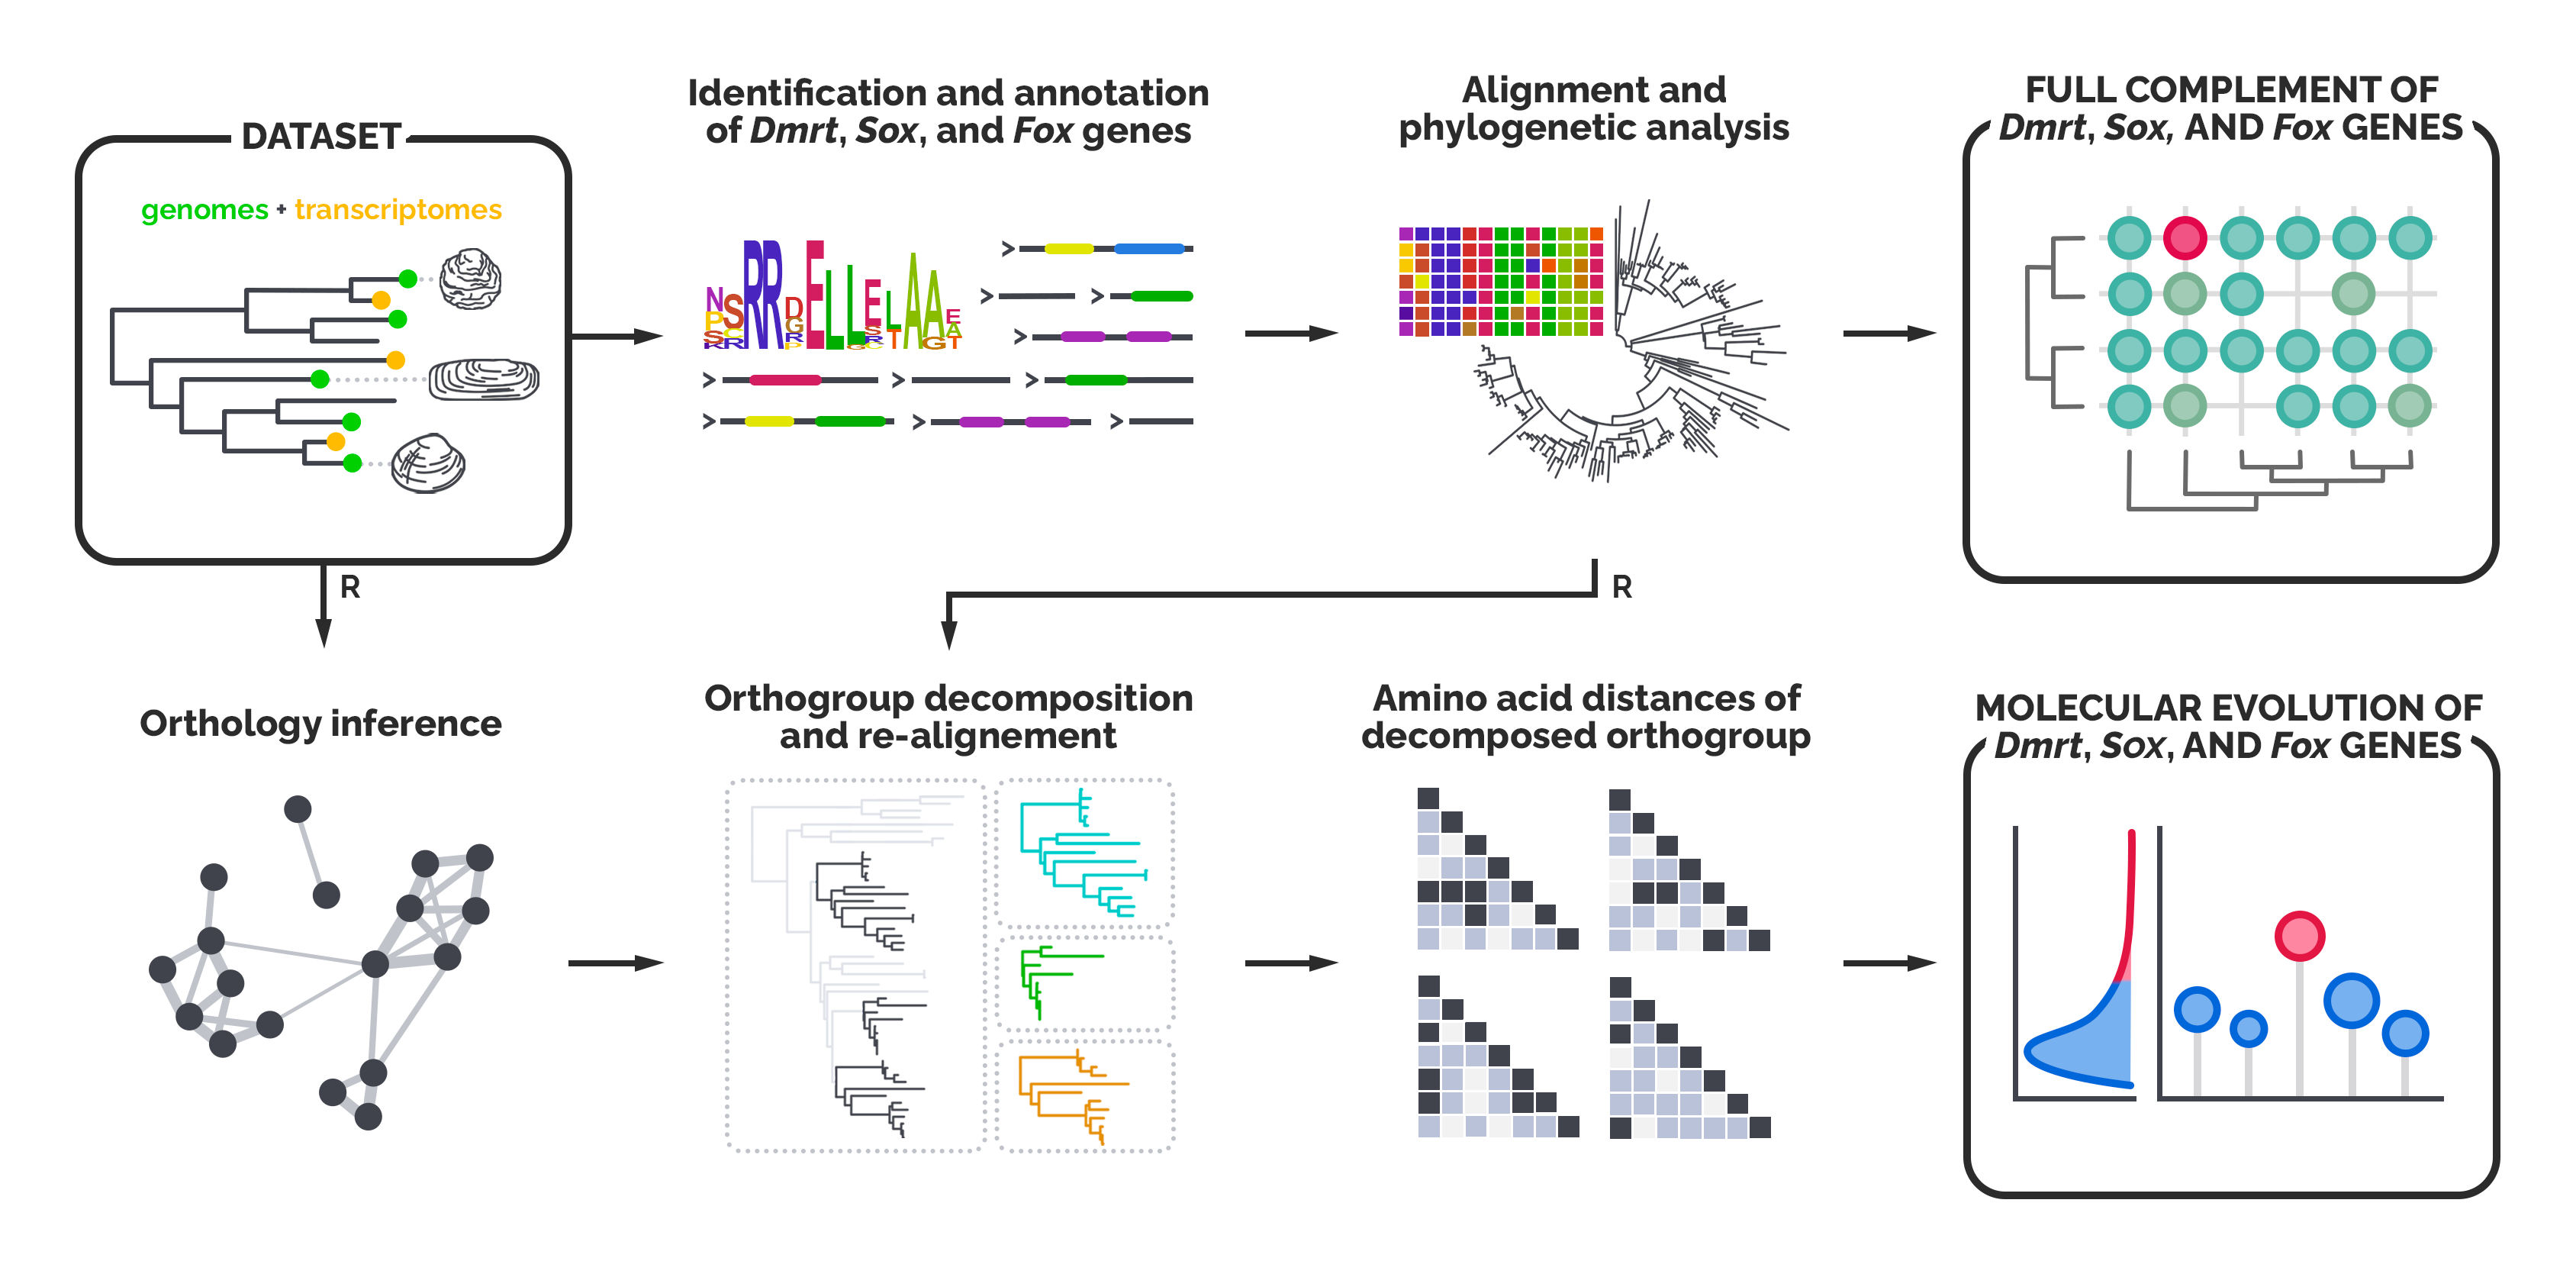
\includegraphics[width=\textwidth]{chapter3/figure_1.png}
    \captionsetup{width=\textwidth}
    \caption{
    \textbf{Workflow of the analyses for the bivalve dataset.} Starting from a set of both genomes and transcriptomes covering a great portion of bivalve taxonomic diversity, we first characterized the entire complement of \textit{Dmrt}, \textit{Sox}, and \textit{Fox} genes (upper row). In particular, we used sequence annotation and phylogenetic tools to obtain reliable sequences and filter out any putative mis-assembled or mis-annotated sequence. Afterwards, we built a reduced set of transcriptomes and genomes (the reduced bivalve dataset, where we minimized the redundancy of congeneric species) from which to draw the molecular evolution patterns of orthologous genes (bottom row). In particular, after having obtained gene single-copy orthologous groups, we calculated the amino acid distances within each orthogroup and then we built the distribution of median values. The same pipeline was also employed for the mammal and the fruit fly datasets, with just two minor differences: the starting dataset was composed of only genomes, and that the reduction step (R) was not necessary.
    }
    \label{fig:workflow}
\end{figure}

\subsection{GO-term enrichment}
After having obtained the distributions of AASD in the three datasets (Bivalvia, Mammalia, and \textit{Drosophila}) and having sorted SCOs genes up into 3 groups (Group 1, group 2, and group 3), we performed a gene ontology (GO) enrichment analysis of genes from Group 1 and genes from Group 1 + Group 2. To do so, we firstly selected one gene per SCO, giving priority to few chosen species: (i) for bivalves, we selected genes from \textit{P. maximus}, or alternatively from \textit{C. gigas}, \textit{Hyriopsis bialata}, \textit{Tridacna squamosa}, and \textit{Solen grandis}; (ii) for mammals, we selected genes from \textit{H. sapiens}, or alternatively from \textit{Bubalus bubalis}, \textit{Panthera tigris}, \textit{Camelus dromedarius}, and \textit{Monodelphis domestica}; (iii) for fruit flies, we selected genes from \textit{D. melanogaster}, or alternatively from \textit{Drosophila ananassae}, \textit{Drosophila hydei}, and \textit{Drosophila suzukii}. By doing so, we ensured that each SCO was represented by one gene. Afterwards, we annotated the obtained datasets with the corresponding GO terms using the OMA browser (accessed 18/09/2024; \textbf{\cite{altenhoff2024oma}}). The GO-term enrichment of Group 1 genes and Group 1 + Group 2 genes was performed with the R package ‘topGO’, using the Fisher exact test (\textbf{\cite{alexa2009gene}}).

\section{Results} \label{chapter3_results}
\subsection{Genomic and transcriptomic datasets}
The complete bivalve dataset consists of 29 bivalve genomes, 14 bivalve transcriptomes, and 7 outgroup genomes (5 gastropods and 2 \textit{Octopus} spp.; \textbf{Supp. Tab. S1}). BUSCO statistics for complete single-copy genes spanned from the 64.9\% in \textit{Modiolus modiolus} to the 99.4\% of \textit{Perna viridis}, with a median value of 94.7\%. We were able to get at least one representative species for 11 different bivalve orders, covering a good proportion of the phylogenetic diversity of the clades Pteriomorphia, Palaeoheterodonta, and Imparidentia, and thus building the most extensive genomic and transcriptomic dataset for bivalve comparative analyses so far (\textbf{Supp. Tab. S1}). Unfortunately, no genomes or transcriptomes for Protobranchia, Archiheterodonta, and Anomalodesmata were available at the time of the project, thus we were not able to include any of those clades in our analysis. The reduced bivalve dataset (used for the orthology inference and the molecular evolution analysis; \textbf{Figure \ref{fig:workflow}}) consists instead of 36 genomes and transcriptomes (\textbf{Supp. Tab. S1}), and was built to retain just one species for each taxonomic genera.

The mammal dataset consists of 32 species and 1 outgroup (\textit{Gallus gallus}, Aves; \textbf{Supp. Tab. S4}), and covers 12 major orders, while the fruit fly dataset consists of 17 species and 1 outgroup (\textit{Anopheles gambiae}, Culicidae; \textbf{Supp. Tab. S5}), and covers 2 \textit{Drosophila} subgenera (i.e., \textit{Drosophila} and \textit{Sophophora}). BUSCO statistics for complete single-copy genes were generally higher than those of bivalves, with a median of 98.3\% for mammals and of 99.8\% for fruit flies (\textbf{Supp. Tab. S4--S5}).

\subsection{The \textit{Dmrt}, \textit{Sox}, and \textit{Fox} complements in bivalves}
Our annotation pipeline managed to successfully identify and annotate DSFGs in bivalves, as proved by the same analysis in mammals and fruit flies (see \textbf{Paragraph \ref{DSFG_test}}).
We retrieved four main orthology groups of \textit{Dmrt} genes in bivalves (\textbf{Figure \ref{fig:DSFG_bivalveCompilation}}; \textbf{Supp. Fig. S1}; \textbf{Supp. Tab. S6}), three corresponding to the groups present in the Bilateria common ancestor (\textit{Dmrt-2}, \textit{Dmrt-3}, and \textit{Dmrt-4/5}; \textbf{\cite{mawaribuchi2019independent}}), and one additional group with no unambiguous ortholog among reference genes, and thus putatively specific to molluscs (named \textit{Dmrt-1L}, as per \textbf{\cite{li2018foxl2,evensen2022comparative}}). The majority of identified \textit{Dmrt} genes are present in single-copy in each species, but \textit{Dmrt-4/5}s show a group-specific expansion in Palaeoheterodonta and Heterodonta, while \textit{Dmrt-1L} is completely absent from Heterodonta. The degree of missing data for \textit{Dmrt} genes in bivalves is about 35\%, with \textit{Dmrt-2} having the highest (about 56\%) and \textit{Dmrt-4/5} the lowest (about 7\%; \textbf{Supp. Tab. S7}). The ubiquitin-binding CUE-like DMA domain has been annotated in most of the \textit{Dmrt-3} and \textit{Dmrt-4/5} genes, while an additional DM domain has been annotated in \textit{Dmrt-1L} genes in Mytilida and the gastropod \textit{Pomacea canaliculata} (\textbf{Supp. Tab. S6}). Additionally, we retrieved six main orthology groups of \textit{Sox} genes, none of which is restricted to molluscs or bivalves (\textbf{Figure \ref{fig:DSFG_bivalveCompilation}}; \textbf{Supp. Fig. S2}; \textbf{Supp. Tab. S6}). Five \textit{Sox} groups (\textit{Sox-B1/2}, \textit{Sox-C}, \textit{Sox-D}, \textit{Sox-E}, and \textit{Sox-F}) are those traditionally considered to be present in the Bilateria common ancestor (\textbf{\cite{phochanukul2010no}}), while one has been identified outside mammals only recently (\textit{Sox-H}, or \textit{Sox-30}; \textbf{\cite{han2010characterization}}). \textit{Sox-B2} and \textit{Sox-B1} have been grouped in the same clade, as in our phylogenetic reconstruction the former results in a paraphyletic group with the latter (\textbf{Supp. Fig. S2}), despite being traditionally recognised as a separate paralogy group in humans, fruit flies, and roundworms. The degree of missing data for \textit{Sox} genes in bivalves is about 8\%, with \textit{Sox-H} having the highest (about 21\%) and \textit{Sox-B1/2} and \textit{Sox-C} both having no missing genes (\textbf{Supp. Tab. S7}). The \textit{Sox} N-terminal signature domain was annotated for \textit{Sox-E} genes (\textbf{Supp. Tab. S6}). Concerning \textit{Fox} genes, we retrieved 27 main orthology groups (\textbf{Figure \ref{fig:DSFG_bivalveCompilation}}; \textbf{Supp. Fig. S3}; \textbf{Supp. Tab. S6}), two of which are specific to molluscs (\textit{Fox-OG13/NA}, \textit{Fox-OG16/NA}). Additionally, other potential mollusc-specific Fox groups have been identified, but these have been excluded from the final orthology analysis as they are present in less than half of bivalve species (see \textbf{Paragraph \ref{chpater3_MM}}; \textbf{Supp. Tab. S6}). The two major \textit{Fox} gene subgroups, Group I (monophyletic, specific to Metazoa; includes \textit{Fox-A}, \textit{Fox-B}, \textit{Fox-C}, \textit{Fox-D}, \textit{Fox-E}, \textit{Fox-F}, \textit{Fox-G}, \textit{Fox-H}, \textit{Fox-L1}, \textit{Fox-L2}, \textit{Fox-Q2}) and Group II (paraphyletic, specific to Opisthokonta; includes \textit{Fox-O}, \textit{Fox-P}, \textit{Fox-J2}, \textit{Fox-J1}, \textit{Fox-K}, \textit{Fox-N2/3}, \textit{Fox-N1/4}; \textbf{\cite{larroux2008genesis}}), have been recovered, including the four \textit{Fox} genes that were present in the Bilateria common ancestor (\textit{Fox-C}, \textit{Fox-F}, \textit{Fox-L1}, and \textit{Fox-Q1}; \textbf{\cite{shimeld2010clustered}}). Two putative lineage-specific expansions have been recovered for \textit{Fox-OG28/NA}, one regarding \textit{Mytilus} spp. and one regarding the two Myida species (\textbf{Figure \ref{fig:DSFG_bivalveCompilation}}; \textbf{Supp. Fig. S3}). The degree of missing data for \textit{Fox} genes in bivalves is about 22\%, with \textit{Fox-H} having the highest (about 42\%) and \textit{Fox-J1} having no missing genes (\textbf{Supp. Tab. S7}). The forkhead-associated (FHA) domain was annotated for \textit{Fox-K} genes, the \textit{Fox-P} coiled-coil signature domain was annotated for \textit{Fox-P} genes, while both the forkhead N- and C-terminal signature domains were annotated for \textit{Fox-A} genes (\textbf{Supp. Tab. S6}).

\begin{figure}
    \centering
    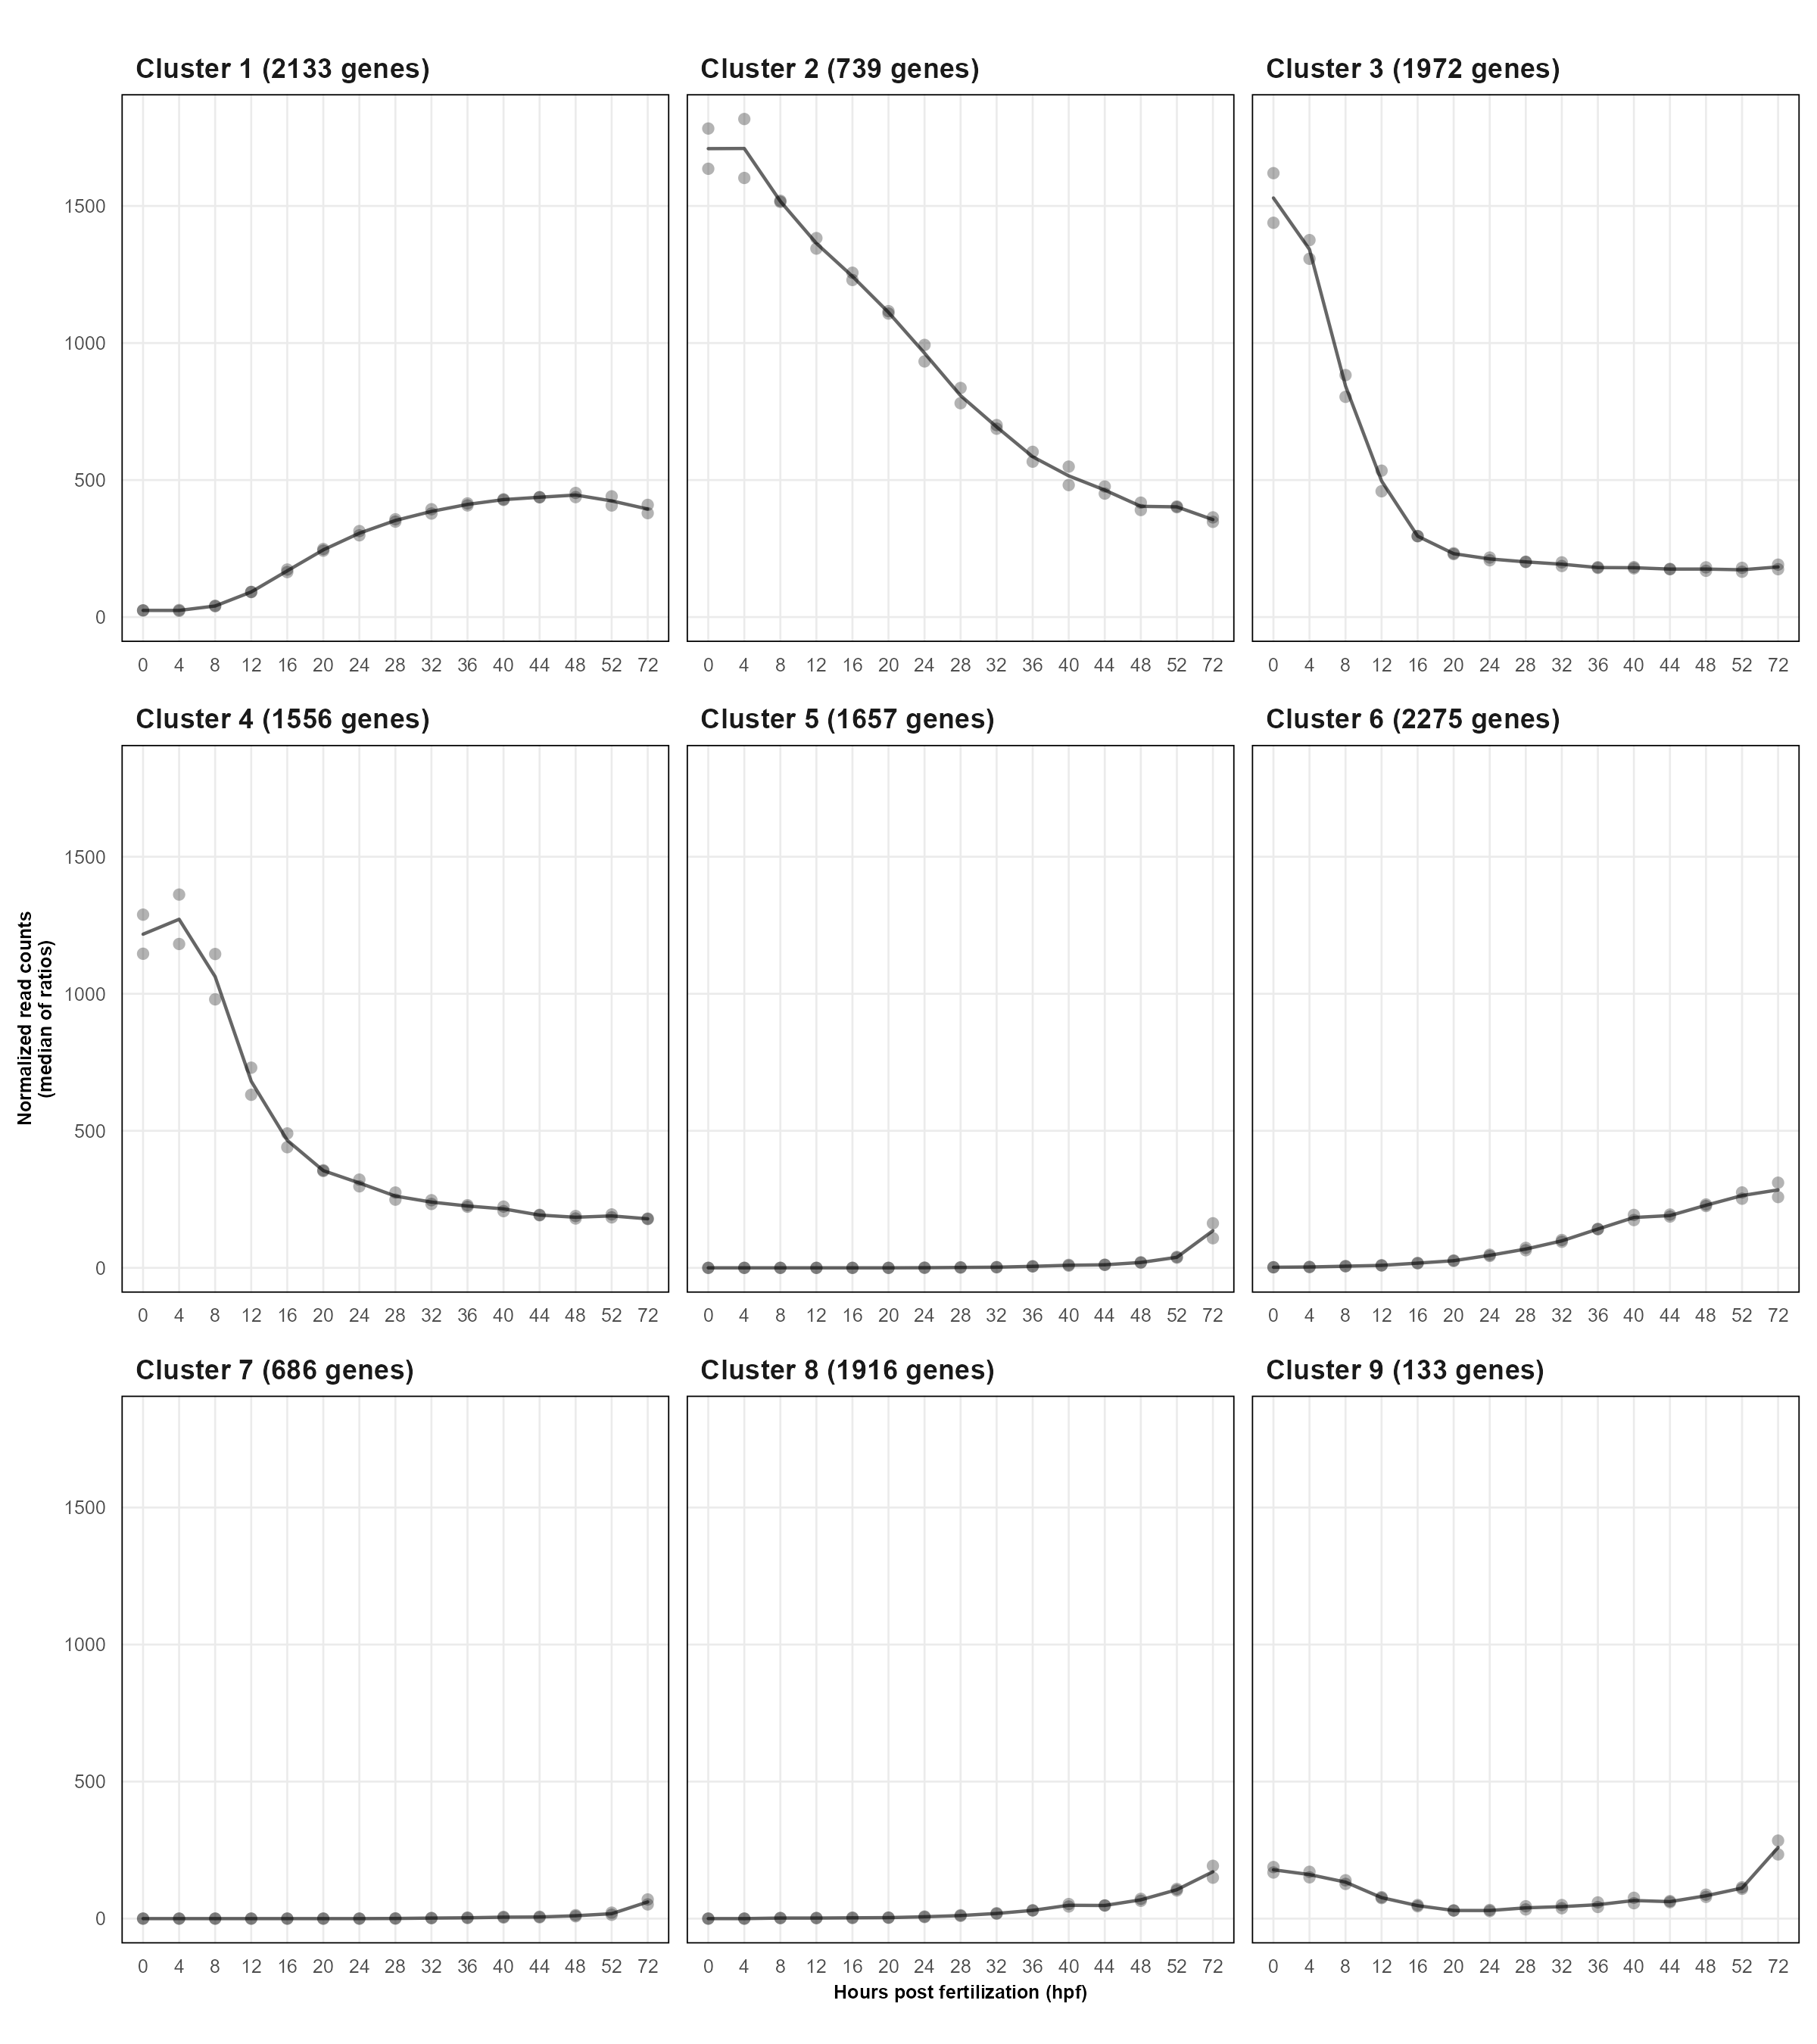
\includegraphics[width=\textwidth]{chapter3/figure_2.png}
    \captionsetup{width=\textwidth}
    \caption{
    \textbf{\textit{Dmrt}, \textit{Sox}, and \textit{Fox} gene (DSFG) complement in bivalves and their outgroups.} Presence/absence of genes in various species are indicated by filled circles. Numbers inside each circle specify genes with 2 or more copies. The shaded area highlights non-bivalve species, belonging either to other molluscs or to the references. The phylogenetic tree of analyzed species, as inferred from literature, is shown on the left, while major taxonomic groups are reported on the right. Species represented by transcriptomic data are marked with an asterisk (‘*’), and species not present in the reduced bivalve dataset are marked with two asterisks (‘**’; see main text and \textbf{Figure \ref{fig:workflow}}); note that the two categories do nor overlap. DSFG trees are shown on the bottom (full trees can be found in \textbf{Supp. Fig. S1--S3}). Full species names, along with all assembly and taxonomic information, can be found in \textbf{Supp. Tab. S1}.  Ad.: Adapedonta; Ar.: Arcida; Ca.: Cardiida; Ce.: Cephalopoda; L.: Lucinida; My.: Myida; Ref.: reference genes; S.: Sphaeriida.
    }
    \label{fig:DSFG_bivalveCompilation}
\end{figure}

Regarding bivalve species, the amount of missing data greatly differs between genomes and transcriptomes, with a mean of about 9\% and about 45\%, respectively. \textit{Argopecten irradians concentricus}, \textit{Mytilus unguiculatus} (\textit{coruscus}), and \textit{Pecten maximus} have no missing data, while \textit{Loripes orbiculatus} has the highest proportion (about 64\%; \textbf{Supp. Tab. S7}).

\subsection{Amino acid sequence divergence of \textit{Dmrt}, \textit{Sox}, and \textit{Fox} genes in bivalves}
In the reduced bivalve dataset, OrthoFinder collectively analysed $>$1.2G genes distributed in 34 species. 89.4\% of these genes were placed in orthogroups, while 10.6\% were not. The number of retrieved SCOs is 5, which is drastically low but can be explained considering the mixed nature of the dataset, that is, it includes both genomes and transcriptomes with highly different BUSCO scores (\textbf{Supp. Tab. S1}). In order to be able to analyse a greater number of genes, we decomposed OrthoFinder orthogroups using DISCO and eventually obtained about 11k SCOs with at least 50\% of the species. By running the same pipeline on DSFGs, we included in the AASD analysis 32 SCOs (\textbf{Figure \ref{fig:DSFG_bivalveCompilation}}) out of 33 initial possvm-identified groups (\textit{Fox-H} didn’t meet the species occupancy threshold; \textbf{Figure \ref{fig:DSFG_bivalveDivergence}}).
From the distribution of median AASD, 112 genes were assigned to Group 1 (1\% upper quantile), 447 to Group 2 (5\% upper quantile), and 10.603 to Group 3. Most of the DSFGs (29/32) fell in Group 3 (\textbf{Figure \ref{fig:DSFG_bivalveDivergence}}), which means they have a median AASD comparable to the vast majority of other genes in bivalves (median level of the genomes). Just \textit{Dmrt-1L}, \textit{Sox-H}, and \textit{Sox-F} showed higher divergences, and have been accordingly placed in Group 2. Overall, pairwise AASD proved to be a good approximation of the tip-to-tip distances (R = 0.84, p < 2.2e\textminus16, calculated on 200 randomly-selected trees; \textbf{Figure \ref{fig:DSFG_bivalveDivergence}C}), while it showed no influence from the alignment length (R = 0.11) or the number of represented species (R =   0.23; \textbf{Figure \ref{fig:DSFG_bivalveDivergence}D--E}). Genes from Group 1 and Group 2 are strongly involved in cellular regulatory processes (such as those related to the metabolism of nucleic acids, proteins, and other macromolecules), but also in development and response to external stimuli, as shown by the GO-term enrichment analysis (\textbf{Table 1}; \textbf{Supp. Tab. S10}).

\begin{figure}
    \centering
    \includegraphics[width=\textwidth]{chapter3/figure_3.png}
    \captionsetup{width=\textwidth}
    \caption{
    \textbf{Distribution of amino acid sequence divergence (AASD) of single-copy orthogroups in bivalves (A), including \textit{Dmrt}, \textit{Sox}, and \textit{Fox} genes (DSFGs; B), and their correlations with tip-to-tip distances (C), alignment lengths (D), and number of species (E).} The distribution of AASD has been computed on the median values of pairwise distances of $>$11k SCOs from the reduced bivalve dataset (see main text and \textbf{Figure \ref{fig:workflow}}). Genes have been divided according to their median AASD value into three different groups, which are indicated by different colors and increasing numbers (Groups 1, 2, and 3). Circle heights of DSFGs show the median value of their AASD, while the size indicates the number of represented species. DSFG trees are shown on the bottom (full trees can be found in \textbf{Supp. Fig. S1--S3}). Darker points in C-E indicate \textit{Dmrt}, \textit{Sox}, and \textit{Fox} gene SCOs. The correlation between the amino acid distance and the tip-to-tip distance has been computed on 200 randomly-selected orthogroups.
    }
    \label{fig:DSFG_bivalveDivergence}
\end{figure}

\subsection{\textit{Dmrt}, \textit{Sox}, and \textit{Fox} genes, and amino acid sequence divergence in the test datasets} \label{DSFG_test}
The DSFG datasets retrieved in mammals and fruit flies are far more complete than those in bivalves, and most of the already-recognised orthology groups have been identified.
In mammals, we retrieved 7 \textit{Dmrt} orthology groups with about 3.1\% of missing data, 20 \textit{Sox} orthology groups with about 8.1\% of missing data, and 42 Fox orthology groups with about 4.6\% of missing data (\textbf{Supp. Fig. S4A, S5--S7}; \textbf{Supp. Tab. S8}). Of these, just \textit{Sox-5} was not included in the subsequent AASD analysis, as it did not meet the 50\%-species occupancy threshold. OrthoFinder analysed circa 650M genes, and the number of SCOs used in the AASD analysis (thus resulting from the DISCO-based orthogroup decomposition pipeline) is $>$16k (\textbf{Figure \ref{fig:DSFG_testDivergence}A}). From the distribution of median AASD, 163 genes were assigned to Group 1, 649 to Group 2, and 15.355 to Group 3. Most of the DSFGs (66/68) fell in Group 3 (Figure \textbf{\ref{fig:DSFG_testDivergence}B}), while \textit{Sry} and \textit{Fox-D4} showed higher divergences, and have been accordingly placed in Group 1 and 2, respectively. Genes from Group 1 and Group 2 show a strong enrichment in immune-related functions (such as innate and adaptive immune response, defence response to bacteria and viruses, lymphocyte methabolism, etc.), but also in reproductive processes (such as  spermatogenesis; \textbf{Tab. \ref{tab:enrichedGOs}}; \textbf{Supp. Tab. S10}).

\begin{landscape}
    \footnotesize
    \begin{longtable}{@{}lllccr@{}}
    \caption{\textbf{Enriched GO terms for Group 1 and Group 2 genes of bivalves, mammals, and Drosophila.} The extended version of the table, which includes also the expected number of annotated genes per GO term and all the other enriched GO terms, can be accessed in \textbf{Supp. Tab. S10}.}
    \label{tab:enrichedGOs}\\
    \toprule
    \multicolumn{1}{c}{\textbf{Dataset}} & \multicolumn{1}{c}{\textbf{GO.ID}} & \multicolumn{1}{c}{\textbf{Term}} & \textbf{\begin{tabular}[c]{@{}c@{}}Annotated\\ genes\end{tabular}} & \textbf{\begin{tabular}[c]{@{}c@{}}Significant\\ genes\end{tabular}} & \multicolumn{1}{c}{\textbf{\begin{tabular}[c]{@{}c@{}}Corrected\\ p-value\end{tabular}}} \\* \hline \hline
    \endfirsthead
    %
    \multicolumn{6}{c}%
    {{\bfseries Table \thetable\ continued from previous page}} \\
    \toprule
    \multicolumn{1}{c}{\textbf{Dataset}} & \multicolumn{1}{c}{\textbf{GO.ID}} & \multicolumn{1}{c}{\textbf{Term}} & \textbf{\begin{tabular}[c]{@{}c@{}}Annotated\\ genes\end{tabular}} & \textbf{\begin{tabular}[c]{@{}c@{}}Significant\\ genes\end{tabular}} & \multicolumn{1}{c}{\textbf{\begin{tabular}[c]{@{}c@{}}Corrected\\ p-value\end{tabular}}} \\* \hline \hline
    \endhead
    %
    \endfoot
    %
    \endlastfoot
    %
    \multirow{21}{*}{\textbf{Bivalvia}} & GO:0060255 & regulation of macromolecule metabolic process & 737 & 59 & 0.04525 \\
     & GO:0080090 & regulation of primary metabolic process & 673 & 53 & 0.01818 \\
     & GO:0019219 & regulation of nucleobase-containing compound metabolic process & 541 & 41 & 0.02388 \\
     & GO:0006351 & DNA-templated transcription & 571 & 39 & 0.03767 \\
     & GO:0032774 & RNA biosynthetic process & 579 & 39 & 0.04490 \\
     & GO:0051252 & regulation of RNA metabolic process & 517 & 37 & 0.02719 \\
     & GO:0006355 & regulation of DNA-templated transcription & 490 & 35 & 0.03751 \\
     & GO:2001141 & regulation of RNA biosynthetic process & 491 & 35 & 0.03844 \\
     & GO:0006950 & response to stress & 370 & 33 & 0.01949 \\
     & GO:0032502 & developmental process & 261 & 27 & 0.04445 \\
     & GO:0006468 & protein phosphorylation & 345 & 23 & 0.02483 \\
     & GO:0031325 & positive regulation of cellular metabolic process & 125 & 17 & 0.00801 \\
     & GO:0010604 & positive regulation of macromolecule metabolic process & 151 & 17 & 0.04047 \\
     & GO:0051172 & negative regulation of nitrogen compound metabolic process & 117 & 16 & 0.00814 \\
     & GO:0051173 & positive regulation of nitrogen compound metabolic process & 137 & 15 & 0.02454 \\
     & GO:0006310 & DNA recombination & 66 & 14 & 0.00087 \\
     & GO:0048513 & animal organ development & 83 & 12 & 0.04088 \\
     & GO:0010629 & negative regulation of gene expression & 78 & 11 & 0.00048 \\
     & GO:0023051 & regulation of signaling & 133 & 11 & 0.02872 \\
     & GO:0045934 & negative regulation of nucleobase-containing compound metabolic process & 64 & 11 & 0.03637 \\
     & GO:0009605 & response to external stimulus & 90 & 11 & 0.04544 \\
    \multirow{1}{*}{\textbf{Bivalvia}} & GO:0044419 & biological process involved in interspecies interaction between organisms & 63 & 11 & 0.04761 \\* \midrule
    \multirow{22}{*}{\textbf{Mammalia}} & GO:0006955 & immune response & 1297 & 145 & 0.00061 \\
     & GO:0098542 & defense response to other organism & 853 & 112 & 0.02066 \\
     & GO:0045087 & innate immune response & 647 & 82 & 8.5e-10 \\
     & GO:0001817 & regulation of cytokine production & 630 & 51 & 0.04660 \\
     & GO:0042742 & defense response to bacterium & 233 & 45 & 1.7e-07 \\
     & GO:0006954 & inflammatory response & 642 & 45 & 0.01735 \\
     & GO:0019221 & cytokine-mediated signaling pathway & 382 & 44 & 3.9e-07 \\
     & GO:0002250 & adaptive immune response & 342 & 44 & 1.3e-05 \\
     & GO:0001819 & positive regulation of cytokine production & 402 & 41 & 0.02723 \\
     & GO:0002697 & regulation of immune effector process & 308 & 37 & 0.04426 \\
     & GO:0042110 & T cell activation & 432 & 35 & 0.02564 \\
     & GO:0051607 & defense response to virus & 257 & 34 & 1.9e-07 \\
     & GO:0048232 & male gamete generation & 491 & 32 & 0.02255 \\
     & GO:0007283 & spermatogenesis & 478 & 31 & 0.02801 \\
     & GO:0070661 & leukocyte proliferation & 273 & 29 & 0.01285 \\
     & GO:0002449 & lymphocyte mediated immunity & 221 & 29 & 0.04833 \\
     & GO:0070663 & regulation of leukocyte proliferation & 212 & 25 & 0.01870 \\
     & GO:0050727 & regulation of inflammatory response & 300 & 24 & 0.00235 \\
     & GO:0031349 & positive regulation of defense response & 240 & 24 & 0.01239 \\
     & GO:0002768 & immune response-regulating cell surface receptor signaling pathway & 177 & 22 & 0.00336 \\
     & GO:0050829 & defense response to Gram-negative bacterium & 66 & 17 & 1.7e-10 \\
     & GO:0071222 & cellular response to lipopolysaccharide & 164 & 17 & 0.00012 \\
     \multirow{13}{*}{\textbf{Mammalia}} & GO:0010466 & negative regulation of peptidase activity & 163 & 16 & 0.00036 \\
     & GO:0002429 & immune response-activating cell surface receptor signaling pathway & 164 & 16 & 0.00243 \\
     & GO:1903555 & regulation of tumor necrosis factor superfamily cytokine production & 137 & 16 & 0.01244 \\
     & GO:0071706 & tumor necrosis factor superfamily cytokine production & 137 & 16 & 0.01244 \\
     & GO:0070665 & positive regulation of leukocyte proliferation & 132 & 16 & 0.02765 \\
     & GO:0045089 & positive regulation of innate immune response & 113 & 16 & 0.03224 \\
     & GO:0071356 & cellular response to tumor necrosis factor & 175 & 15 & 0.00219 \\
     & GO:0002695 & negative regulation of leukocyte activation & 148 & 15 & 0.01151 \\
     & GO:0002456 & T cell mediated immunity & 82 & 15 & 0.01605 \\
     & GO:0002705 & positive regulation of leukocyte mediated immunity & 113 & 15 & 0.01837 \\
     & GO:0032680 & regulation of tumor necrosis factor production & 133 & 15 & 0.03262 \\
     & GO:0032640 & tumor necrosis factor production & 133 & 15 & 0.03262 \\
     & GO:0050866 & negative regulation of cell activation & 165 & 15 & 0.04048 \\* \midrule
    \multirow{10}{*}{\textit{\textbf{Drosophila}}} & GO:0000819 & sister chromatid segregation & 140 & 11 & 0.02927 \\
     & GO:0070192 & chromosome organization involved in meiotic cell cycle & 54 & 9 & 0.00849 \\
     & GO:0007131 & reciprocal meiotic recombination & 37 & 7 & 0.00066 \\
     & GO:0007143 & female meiotic nuclear division & 54 & 6 & 0.02270 \\
     & GO:0035967 & cellular response to topologically incorrect protein & 44 & 5 & 0.03334 \\
     & GO:0035966 & response to topologically incorrect protein & 47 & 5 & 0.04266 \\
     & GO:0007141 & male meiosis I & 13 & 4 & 0.00150 \\
     & GO:0140543 & positive regulation of piRNA transcription & 3 & 3 & 6.9e-05 \\
     & GO:0010526 & retrotransposon silencing & 8 & 3 & 0.00331 \\
     & GO:0007130 & synaptonemal complex assembly & 10 & 3 & 0.00666 \\
     \multirow{5}{*}{\textit{\textbf{Drosophila}}} & GO:0030719 & P granule organization & 11 & 3 & 0.00888 \\
     & GO:0071218 & cellular response to misfolded protein & 12 & 3 & 0.01149 \\
     & GO:0051788 & response to misfolded protein & 12 & 3 & 0.01149 \\
     & GO:0007135 & meiosis II & 15 & 3 & 0.02169 \\
     & GO:0034508 & centromere complex assembly & 19 & 3 & 0.04094 \\* \bottomrule \bottomrule
    \end{longtable}
    \end{landscape}

Concerning \textit{Drosophila}, we retrieved 4 \textit{Dmrt} orthology groups with about 1.7\% of missing data, 7 \textit{Sox} orthology groups with about 3.9\% of missing data, and 17 \textit{Fox} genes with about 8.3\% of missing data (\textbf{Supp. Fig. S4B, S9--S10}; \textbf{Supp. Tab. S9}). OrthoFinder analysed about 240M, and the distribution of median AASD was built after $>$12k SCOs (\textbf{Figure \ref{fig:DSFG_testDivergence}C}). 126 genes were assigned to Group 1, 501 to Group 2, and 11.880 to Group 3. All of the DSFGs have been used in the AASD analysis, but none of them have been placed in Group 1 or 2, that is, all the DSFGs in \textit{Drosophila} have an AASD comparable to the median level of the genome (\textbf{Figure \ref{fig:DSFG_testDivergence}D}). Genes of Group 1 and Group 2 show a GO-term enrichment in meiotic processes, such as chromosome/chromatid organisation, and retrotransposon silencing (\textbf{Table 1}; \textbf{Supp. Tab. S10}).

\begin{figure}
    \centering
    \includegraphics[width=0.9\textwidth]{chapter3/figure_4.png}
    \captionsetup{width=\textwidth}
    \caption{
    \textbf{Distribution of amino acid divergence (AASD) of single-copy orthogroups in Mammalia (A) and \textit{Drosophila} (C), including \textit{Dmrt}, \textit{Sox}, and \textit{Fox} genes (DSFGs; B-D).} The distributions of AASD in mammals and fruit flies have been computed on the median values of pairwise distances of over 16k and 12k SCOs, respectively. Genes have been divided according to their median AASD value into three different groups, which are indicated by different colors and increasing numbers (Groups 1, 2, and 3). Circle heights of DSFGs show the median value of their AASD, while the size indicates the number of represented species. DSFG trees are shown on the bottom (full trees can be found in \textbf{Supp. Fig. S5--S7} for mammals and in \textbf{Supp. Fig. S8--S10} for fruit flies). Insets: scheme of the sex-determination molecular pathways in \textit{Mus musculus} and in \textit{Drosophila melanogaster}, with shown the main genes involved (adapted from \textbf{\cite{beukeboom2014evolution}}). Green arrows indicate transcription activations, red arrows indicate transcription suppressions. X: sex chromosomes; A: autosomal chromosomes; \textit{DSX\textsuperscript{M/F}}: \textit{DSX} splicing variants present in males or females, respectively.
    }
    \label{fig:DSFG_testDivergence}
\end{figure}

\section{Discussion} \label{chpater3_discussion}
\subsection{A new manually-curated and phylogenetic-based reference dataset of \textit{Dmrt}, \textit{Sox}, and \textit{Fox} genes in bivalves}

The annotation and characterization process of a gene family in a certain clade of organisms may harbour many overlooked challenges (\textbf{\cite{vizueta2020bitacora}}). For example, the presence of highly-conserved catalytic domains may hamper the correct identification of the components of a gene family, as it is the case for \textit{Hox} and \textit{ParaHox} genes and their homeobox motif (\textbf{\cite{nicolini2023comparative,baldwin2018new}}). Conversely, the components of dynamic gene families characterised by abrupt and sequential duplication events may be difficult to sort into separate groups. As a matter of fact, varying levels of sequence heterogeneity and of gene copy numbers makes the inference of orthologous groups hard, as for certain P450 clans (\textbf{\cite{dermauw2020diversity}}). Regardless of the causes, having a solid and wide phylogenetic context in which to study gene duplications and losses, and orthology relationships, is crucial to overcome these difficulties. In the same way, manual curation and visual inspection of multiple sequence alignments, phylogenetic trees, and gene structures (in terms of domain annotation, start and stop codons, and other feature representations) is helpful, despite being time-demanding and possibly low reproducible. In this study, we characterised the full complement of DSFGs in the vast clade of bivalves, by leveraging sequence domain annotation, phylogenetics, and manual curation of the dataset. Our aim was to obtain the most reliable gene complements as possible, combined with a vast taxonomic dataset, a solid phylogenetic inference, an openly-available dataset of gene sequences, and a reproducible pipeline for the annotation of gene identity. By doing so, we want to provide a reliable resource for future studies of DSFGs, either focused on bivalves or generally in Metazoa.

Our approach allowed us to identify some cases of incorrect gene identification and relative nomenclature in bivalves, which have arisen because of erroneous or ambiguous annotations in previous works, as a result of limited datasets or analyses. For example, concerning the \textit{Dmrt} gene family, we identified orthologs of the vertebrate \textit{Dmrt-2}, \textit{Dmrt-3}, and \textit{Dmrt-4/5} (\textit{A1/A2}; \textbf{Figure \ref{fig:DSFG_bivalveCompilation}}; \textbf{Supp. Fig. S1}; \textbf{Supp. Tab. S6}), which are also expected to have been present in the Bilateria common ancestor (\textbf{\cite{mawaribuchi2019independent}}). \textbf{\cite{wang2023genome}} found that \textit{Dmrt-4/5} is duplicated in \textit{Mercenaria mercenaria} and \textit{Cyclina sinensis} (Venerida), and in \textit{Dreissena polymorpha} (Myida), and we confirm this result by tracing back the duplication event to the split between Palaeoheterdonta (here represented by Unionida) and Heterodonta (here represented by Venerida, Myida, Sphaeriida, Adapedonta, Cardiida, and Lucinida; \textbf{Figure \ref{fig:DSFG_bivalveCompilation}}). Furthermore, we confirm \textit{Dmrt-1L} to be present in many bivalve species (mainly belonging to the Ostreida, Pectinida, Mytilida, and Unionida orders; \textbf{Figure \ref{fig:DSFG_bivalveCompilation}}), as well as in gastropods and \textit{Octopus}. Though, our phylogenetic analysis did not retrieve any unambiguous orthology relationship among \textit{Dmrt-1L} and either vertebrate \textit{Dmrt-1} or \textit{Drosophila} \textit{dsx} genes, as instead it was proposed in previous works (\textbf{\cite{li2018foxl2,evensen2022comparative}}). As a matter of fact, the amino acid sequence of the \textit{Dmrt-1L} DM domain does not recall that of any other \textit{Dmrt} gene. Furthermore, it must be considered that various phylogenetic analyses have recovered both \textit{Dmrt-1} and \textit{dsx} genes to be restricted to vertebrates and arthropods, respectively (\textbf{\cite{wexler2014pan,mawaribuchi2019independent,panara2019phylogenetic}}), that is, they do not have any direct ortholog outside their relative clades. Thus, if \textit{Dmrt-1L}, \textit{dsx}, and \textit{Dmrt-1} are true orthologs, their origin would need to be placed at least in the Bilateria common ancestor, which seems however to not be the case. All considered, we thus confirm that \textit{Dmrt-1L} is not homologous to \textit{Dmrt-1} and \textit{Dsx} and is rather a mollusc-specific gene (\textbf{\cite{evensen2022comparative}}). The monophyly of the group, which is not supported by the phylogenetic tree inferred with Dmrt genes from also the reference species (\textbf{Supp. Fig. S1}), is instead recovered when analysing just genes from mollusc species (Supp Fig. S11). To this regard, we speculate that in our analysis, the difficulty in obtaining the monophyly of \textit{Dmrt-1L} genes may have arisen primarily because of the many \textit{C. elegans}-restricted genes (\textbf{Supp. Tab. S3}), which are placed among the other bivalve genes (\textbf{Supp. Fig. S1}), but also because of the high AASD of \textit{Dmrt-1L} genes (see High amino acid sequence divergence and identification of sex-determining genes LINK LINK LINK), which hampers a straight-forward phylogenetic reconstruction. Our broad-context analysis also suggests that (i) the scallop-specific cluster of Dmrt genes retrieved by \textbf{\cite{wang2023genome}} rather belongs to the \textit{Dmrt-1L} group, and (ii) the classification of \textit{Dmrt} genes of bivalves provided by \textbf{\cite{zeng2024genome}} needs to be revised as proposed in this work (for example, \textit{Dmrt-1} genes are \textit{Dmrt-4/5}; \textit{Dmrt-2} genes are \textit{Dmrt-3}; \textit{Dmrt-3} genes are \textit{Dmrt-1L}; hence, Crassostrea species do not have \textit{Dmrt-2} genes).

For what concerns the \textit{Sox} gene family, bivalves (or molluscs) do not show any major clade-restricted gene, as only the five Bilateria-specific \textit{Sox} groups (\textit{Sox-B1/2}, \textit{Sox-C}, \textit{Sox-D}, \textit{Sox-E}, and \textit{Sox-F}) and \textit{Sox-H} have been mainly identified (\textbf{Figure \ref{fig:DSFG_bivalveCompilation}}; \textbf{Supp. Fig. S2}; \textbf{Supp. Tab. S6}), in accordance with previous findings (\textbf{\cite{yu2017genome,evensen2022comparative,wang2024genome}}). \textit{Sox-B1/2} is clearly made up of two subgroups (i.e., \textit{Sox-B1} and \textit{Sox-B2}), as expected, but their respective identity could not be unambiguously established, as \textit{Sox-B1/2} genes of reference species do not form separate clusters (\textbf{Supp. Fig. S2}). Even when inferring the phylogenetic tree only of components of the \textit{Sox-B1/2} group from molluscs and reference species, the identity can not be established properly (\textbf{Supp. Fig. S12}).

Compared to \textit{Dmrt} and \textit{Sox} genes, the \textit{Fox} gene family appears as the most dynamic in terms of gene presence/absence, as already shown by other works (\textbf{\cite{wu2020identification,schomburg2022phylogenetic,seudre2022fox}}). Our phylogenetic analysis successfully recovered Group I and Group II of \textit{Fox} genes (\textbf{\cite{larroux2008genesis}}), which include the four \textit{Fox} genes that were present in the Bilateria common ancestor (\textit{Fox-C}, \textit{Fox-F}, \textit{Fox-L1}, and \textit{Fox-Q1}; \textbf{Figure \ref{fig:DSFG_bivalveCompilation}}; \textbf{Supp. Fig. S3}; \textbf{Supp. Tab. S6}; \textbf{\cite{shimeld2010clustered}}). To our knowledge, this is the first broad-taxonomic identification and classification of \textit{Fox} genes in bivalves, as up to now they have been systematically characterised only in \textit{Crassostrea gigas} (\textbf{\cite{yang2014phylogeny}}), \textit{Patinopecten yessoensis} (\textbf{\cite{wu2020identification}}), and \textit{Ruditapes philippinarum} (\textbf{\cite{liu2024characterization}}). Firstly, our analysis confirms the absence in molluscs of \textit{Fox-I}, \textit{Fox-Q1}, \textit{Fox-R}, \textit{Fox-S} (\textbf{Supp. Fig. S3}), which are in fact thought to have emerged with the diversification of deuterostomes or vertebrates (\textbf{\cite{yang2014phylogeny,wu2020identification,schomburg2022phylogenetic,seudre2022fox}}). Furthermore, we found many \textit{Fox} groups that appeared as mollusc-specific and/or still-unnamed at a first analysis. However, a much more in-depth investigation revealed a different scenario. \textit{Fox-OG2/NA} appears close to the human \textit{Fox-M} gene in the phylogenetic tree, but they do not form a monophyletic group (\textbf{Supp. Fig. S3}). However, by comparing \textit{Fox-OG2/NA} sequences and the phylogenetic tree with those analysed by \textbf{\cite{yang2014phylogeny}}, \textbf{\cite{wu2020identification}}, \textbf{\cite{schomburg2022phylogenetic}}, \textbf{\cite{seudre2022fox}}, it appears clear that this group of \textit{Fox} genes is indeed \textit{Fox-M}. However, our analysis has failed to retrieve a monophyletic relationship among bivalve and human \textit{Fox-M} genes, even when inferring a tree with just \textit{Fox-J2}, \textit{Fox-M}, \textit{Fox-O}, and \textit{Fox-P} complements (\textbf{Supp. Fig. S13}), which belong to the same \textit{Fox} group. Regarding the \textit{Fox-OG39/NA} group, it does not have any homolog in reference species (\textbf{Supp. Fig. S3}) but is found to belong to the \textit{Fox-AB} group by sequence comparison with previous works (\textbf{\cite{yang2014phylogeny,wu2020identification,seudre2022fox}}). \textit{Fox-AB} was formerly described only in the sea urchin \textit{Strongylocentrotus purpuratus} and the lancelet \textit{Branchiostoma floridae} (\textbf{\cite{yu2008fox,tu2006sea}}), but was later identified also in several Spiralia lineages, including molluscs (e.g., \textbf{\cite{yang2014phylogeny,wu2020identification,seudre2022fox}}). A similar situation concerns \textit{Fox-OG15/NA} and \textit{Fox-OG28/NA}, which again could not be named based on orthology relationships with the reference species genes (\textbf{Supp. Fig. S3}), but actually represent two lineage-specific expansions of the \textit{Fox-Q2} group (named \textit{Fox-Q2b} and \textit{Fox-Q2c}), as already appointed in previous studies (\textbf{\cite{yang2014phylogeny,wu2020identification}}). This observation fits within the wider context of the \textit{Fox-Q2} group expansion in Bilateria and, particularly, in Spiralia, that led to remarkable differences in their gene copy numbers across various clades (\textbf{\cite{seudre2022fox}}). Two additional \textit{Fox} genes have been previously identified in bivalves, and were named \textit{Sox-Y} and \textit{Sox-Z} (\textbf{\cite{yang2014phylogeny,wu2020identification}}). In our analysis, these \textit{Fox} groups were identified as \textit{Fox-OG13/NA} and \textit{Fox-OG16/NA}, thanks to sequence comparison of \textit{Fox} genes from \textit{C. gigas} and \textit{P. yessoensis}. On one hand, \textit{Fox-Y} was firstly identified in \textit{S. purpuratus} (\textbf{\cite{tu2006sea}}) and only recently in a few bivalve species (\textbf{\cite{yang2014phylogeny,wu2020identification}}). However, when analysing bivalve and \textit{S. purpuratus} \textit{Fox} genes, we failed in retrieving such a clear orthology relationship, as \textit{S. purpuratus} \textit{Fox-Y} does not fall within the phylogenetic range of bivalve \textit{Fox-OG13/NA}, which contains the supposed \textit{Fox-Y} orthologs (\textbf{Supp. Fig. S14}). Also, the forkhead domains of \textit{Fox-OG13/NA} genes were annotated as ‘forkhead domain P’ (\textbf{Supp. Fig. S6}). On the other hand, \textit{Fox-Z} was firstly identified in bivalves and in several other protostomes, thanks to a phylogenetic work including the brachiopod \textit{Lingula unguis}, the annelid \textit{Capitella teleta}, the scorpion \textit{Centruroides sculpturatus}, and the centipede \textit{Strigamia maritima} (\textbf{\cite{wu2020identification}}). However, later works have not recovered this result, even when analysing annelids (\textbf{\cite{seudre2022fox}}) and panarthropods (\textbf{\cite{schomburg2022phylogenetic}}) in a more focused effort. In this case, the forkhead domains were annotated as either a generic ‘forkhead domain’ or a ‘forkhead domain Q2’ (\textbf{Supp. Fig. S6}). All considered, we argue that bivalves possess two additional \textit{Fox} groups (here \textit{Fox-OG13/NA} and \textit{Fox-OG16/NA}; \textbf{Figure \ref{fig:DSFG_bivalveCompilation}}; \textbf{Supp. Fig. S3}; \textbf{Supp. Tab. S6}) which are shared with other mollusc species, as revealed also by other authors. However, given the discordant results of the phylogenetic hypothesis and domain annotation, we think that a more thorough investigation on their orthology relationships with \textit{Fox} genes from other Metazoa is needed, and thus we chose to not employ their former names \textit{Fox-Y} and \textit{Fox-Z}.

Besides the DSFG groups discussed so far, it must be also considered that many orphan genes have been identified (\textbf{Supp. Fig. S1--S3}; \textbf{Supp. Tab. S6}). For example, \textbf{\cite{wu2020identification}} identified a duplication event of \textit{Fox-H} genes in \textit{C. gigas}, which has been recovered also in our analysis for the entire Ostreida clade (\textit{Fox-OG36/NA}; \textbf{Supp. Fig. S3}). Similarly, a gene orthology group putatively specific to Pteriomorphia has been identified among \textit{Sox} genes (\textit{Sox-OG1/NA}). Of course, these genes deserve as much attention as the others, as they may constitute true group-specific expansions and may play fundamental roles in some biological processes. However, they have not been discussed here or included in \textbf{Figure \ref{fig:DSFG_bivalveCompilation}} for clarity purposes, but they are freely available in supplementary materials.

Overall, our analysis clearly shows the importance of adopting a wide-angle approach when characterising the members of a gene family, especially for large ones such as the Fox genes (\textbf{\cite{schomburg2022phylogenetic}}). As a matter of fact, the presence of duplication events and orphan genes needs to be addressed with a broad taxonomic dataset, in order to account for possible mis-annotations, gene phylogenetic mis-placements, and sequence heterogeneity. Additionally, many reference species need to be included for the gene identification process, in order to consider distantly-related genes and obtain a solid annotation. Our gene annotation pipeline also resulted to be very solid, even with non-model organisms and sub-optimal genomic and transcriptomic resources as they are those of bivalves. As a matter of fact, by running the same pipeline on two additional datasets composed of mammal and fruit fly genomes, we were able to obtain high-quality orthology groups in accordance with previous knowledge on the clades (\textbf{Supp. Fig. S4--S10}; \textbf{Supp. Tab. S8--S9}), with little or no manual curation. Furthermore, this is again the first broad analysis of DSFGs in both mammals and fruit flies, as so far attention has been dedicated only to single well-studied organisms (e.g., \textbf{\cite{jackson2010update}}).

\section{Conclusions.} \label{chapter3_conclusions}

\textbf{\textit{In preparation.}}

\section{Supplementary Materials} \label{chapter3_supp}

\textit{All the supplementary materials will be available at my GitHub personal page.}

\subsection*{Supplementary Figures}

\small{

    \textbf{Supplementary Figure S1. ML phylogenetic tree of the \textit{Dmrt} gene family in molluscs, including the possvm orthology inference.} Reference genes from \textit{H. sapiens}, \textit{C. elegans}, and \textit{D. melanogaster} are marked with an asterisk at the beginning of the tip names. Species ID can be found in \textbf{Supp. Tab. S1}. The tree has been midpoint rooted. Bootstrap values are shown for each node.

    \vspace{5mm}

    \noindent\textbf{Supplementary Figure S2. ML phylogenetic tree of the \textit{Sox} gene family in molluscs, including the possvm orthology inference.} Reference genes from \textit{H. sapiens}, \textit{C. elegans}, and \textit{D. melanogaster} are marked with an asterisk at the beginning of the tip names. Species ID can be found in \textbf{Supp. Tab. S1}. Bootstrap values are shown for each node.

    \vspace{5mm}

    \noindent\textbf{Supplementary Figure S3. ML phylogenetic tree of the \textit{Fox} gene family in molluscs, including the possvm orthology inference.} Reference genes from \textit{H. sapiens}, \textit{C. elegans}, and \textit{D. melanogaster} are marked with an asterisk at the beginning of the tip names. Species ID can be found in \textbf{Supp. Tab. S1}. Bootstrap values are shown for each node.
    
    \vspace{5mm}

    \noindent\textbf{Supplementary Figure S4. \textit{Dmrt}, \textit{Sox}, and \textit{Fox} gene (DSFG) complement in Mammalia and \textit{Drosophila} spp.} Presence/absence of genes in various species are indicated by filled circles. Numbers inside each circle specify genes with 2 or more copies. The shaded area highlights outgroup species, \textit{Gallus gallus} (Aves) for mammals and \textit{Anopheles gambiae} (Culicidae) for fruit flies. The phylogenetic tree of analysed species, as inferred from literature, is shown on the left, while major taxonomic groups are reported on the right. All species are represented by genomic data. DSFG trees are shown on the bottom (full trees can be found in \textbf{Supp. Fig. S5--S7}). Full species names for both mammals and fruit flies, along with all assembly and taxonomic information, can be found in \textbf{Supp. Tab. S4} and \textbf{Supp. Tab. S5}, respectively. A.: Aves; Chirop.: Chiroptera; L.: Lagomorpha; M.: Monotremata; Me.: Metatheria; P.: Pholidota; Pe.: Perissodactyla; Prim.: Primates; Roden.: Rodentia; X.: Xenarthra; C.: Culicidae.
    
    \vspace{5mm}

    \noindent\textbf{Supplementary Figure S5. ML phylogenetic tree of the Dmrt gene family in mammals, including the possvm orthology inference.} Reference genes from \textit{H. sapiens}, \textit{Mus musculus}, \textit{Elephas maximus indicus}, and \textit{Ornithorhynchus anatinus} are marked with an asterisk at the beginning of the tip names. Species ID can be found in \textbf{Supp. Tab. S4}. The tree has been midpoint rooted. Bootstrap values are shown for each node.
    
    \vspace{5mm}

    \noindent\textbf{Supplementary Figure S6. ML phylogenetic tree of the \textit{Sox} gene family in mammals, including the possvm orthology inference.} Reference genes from \textit{H. sapiens}, \textit{Mus musculus}, \textit{Elephas maximus indicus}, and \textit{Ornithorhynchus anatinus} are marked with an asterisk at the beginning of the tip names. Species ID can be found in \textbf{Supp. Tab. S4}. Bootstrap values are shown for each node.
    
    \vspace{5mm}

    \noindent\textbf{Supplementary Figure S7. ML phylogenetic tree of the \textit{Fox} gene family in mammals, including the possvm orthology inference.} Reference genes from \textit{H. sapiens}, \textit{Mus musculus}, \textit{Elephas maximus indicus}, and \textit{Ornithorhynchus anatinus} are marked with an asterisk at the beginning of the tip names. Species ID can be found in \textbf{Supp. Tab. S4}. Bootstrap values are shown for each node.
    
    \vspace{5mm}

    \noindent\textbf{Supplementary Figure S8. ML phylogenetic tree of the \textit{Dmrt} gene family in fruit flies, including the possvm orthology inference.} Reference genes from \textit{D. melanogaster}, \textit{Drosophila hydei}, \textit{Drosophila pseudoobscura}, and \textit{Drosophila suzukii} are marked with an asterisk at the beginning of the tip names. Species ID can be found in \textbf{Supp. Tab. S5}. The tree has been midpoint rooted. Bootstrap values are shown for each node.

    \vspace{5mm}

    \noindent\textbf{Supplementary Figure S9. ML phylogenetic tree of the \textit{Sox} gene family in fruit flies, including the possvm orthology inference.} Reference genes from \textit{D. melanogaster}, \textit{Drosophila hydei}, \textit{Drosophila pseudoobscura}, and \textit{Drosophila suzukii} are marked with an asterisk at the beginning of the tip names. Species ID can be found in \textbf{Supp. Tab. S5}. Bootstrap values are shown for each node.

    \vspace{5mm}

    \noindent\textbf{Supplementary Figure S10. ML phylogenetic tree of the \textit{Fox} gene family in fruit flies, including the possvm orthology inference.} Reference genes from \textit{D. melanogaster}, \textit{Drosophila hydei}, \textit{Drosophila pseudoobscura}, and \textit{Drosophila suzukii} are marked with an asterisk at the beginning of the tip names. Species ID can be found in \textbf{Supp. Tab. S5}. Bootstrap values are shown for each node.

    \vspace{5mm}

    \noindent\textbf{Supplementary Figure S11. ML phylogenetic tree of the \textit{Dmrt} gene family in mollusc species.} Species ID can be found in \textbf{Supp. Tab. S1}. The tree has been midpoint rooted. Bootstrap values are shown for each node.

    \vspace{5mm}

    \noindent\textbf{Supplementary Figure S12. ML phylogenetic tree of \textit{Fox-J2}, \textit{Fox-M}, \textit{Fox-O}, and \textit{Fox-P} genes in mollusc and reference species.} Reference genes from \textit{H. sapiens}, \textit{C. elegans}, and \textit{D. melanogaster} are marked with an asterisk at the beginning of the tip names. Species ID can be found in \textbf{Supp. Tab. S1}. Bootstrap values are shown for each node.

    \vspace{5mm}

    \noindent\textbf{Supplementary Figure S13. ML phylogenetic tree of \textit{Fox-J2}, \textit{Fox-M}, \textit{Fox-O}, and \textit{Fox-P} genes in mollusc and reference species.} Reference genes from \textit{H. sapiens}, \textit{C. elegans}, and \textit{D. melanogaster} are marked with an asterisk at the beginning of the tip names. Species ID can be found in \textbf{Supp. Tab. S1}. Bootstrap values are shown for each node.

    \vspace{5mm}

    \noindent\textbf{Supplementary Figure S14. ML phylogenetic tree of the \textit{Fox} gene family in bivalves and the sea urchin \textit{Strongylocentrotus purpuratus} (Spur).} Reference genes from \textit{S. purpuratus} are marked with an asterisk at the beginning of the tip names. Species ID can be found in \textbf{Supp. Tab. S1}. \textit{S. purpuratus} genes are those given by \textbf{\cite{tu2006sea}}. Bootstrap values are shown for each node.

    \vspace{5mm}
    
    \noindent\textbf{Supplementary Figure S15. Distribution of amino acid divergence (AASD) of single-copy orthogroups in \textit{Crassostrea} species (\textit{Crassostra gigas}, \textit{Crassostrea angulata}, \textit{Csrassostrea ariakensis}, and \textit{Crassostrea virginica}; A), including \textit{Dmrt}, \textit{Sox}, and \textit{Fox} genes (DSFGs; B).} The distribution of AASD in \textit{Crassostrea} has been computed on the median values of pairwise distances of over 14k SCOs. Circle heights of DSFGs show the median value of their AASD. \textit{Dmrt-1L} genes are indicated as ‘dmrt\_disco\_tree3’.
}

\section*{Supplementary Tables}

\textbf{\textit{In preparation.}}

\end{document}